\documentclass[border=2pt]{standalone}
\usepackage[T1]{fontenc}
\usepackage[tt=false]{libertine}
\usepackage[libertine]{newtxmath}
\usepackage[varqu]{zi4}
\usepackage{tikz}
\usetikzlibrary{positioning,arrows.meta,shapes.geometric,shapes.symbols,calc,fit,backgrounds}
% paper \textwidth (acmart sigconf) = 506.295pt; every variant is drawn to fit it at \small (8pt)
\newcommand{\tw}{506pt}

\begin{document}\small
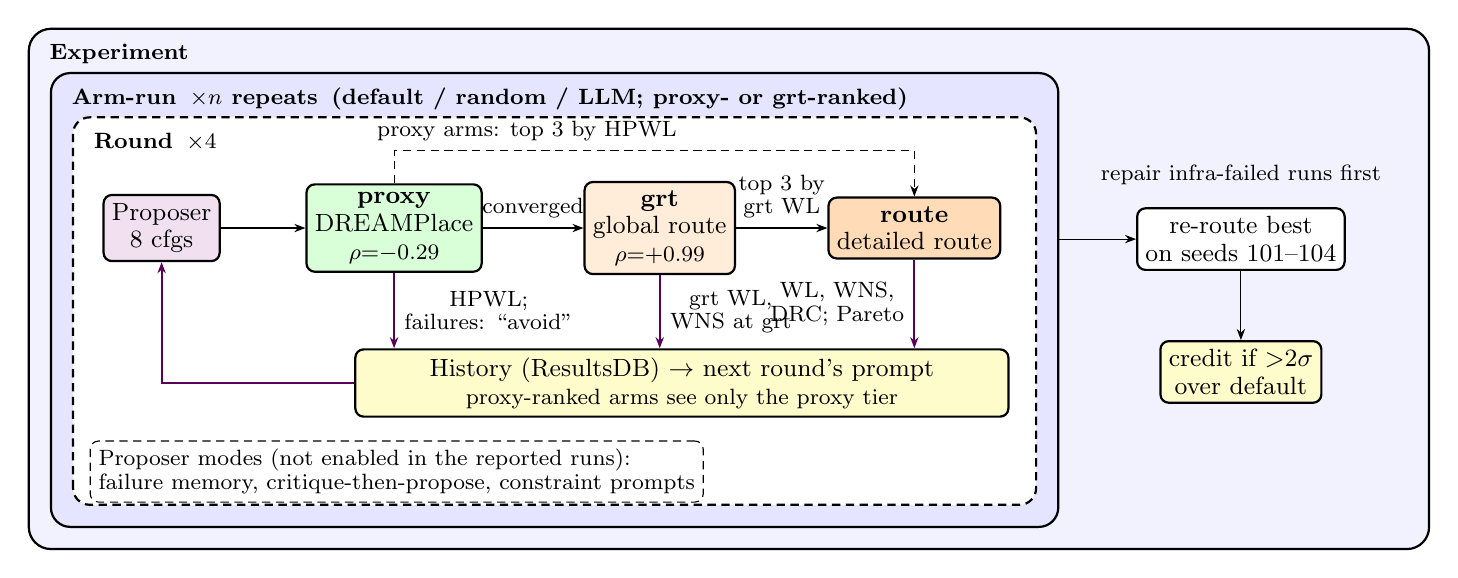
\begin{tikzpicture}[x=1pt,y=1pt,>={Stealth[length=4pt]},
  b/.style={draw,thick,rounded corners=3pt,align=center,inner sep=3pt,minimum height=22pt,fill=white,font=\small},
  lab/.style={font=\footnotesize,align=center},
  fb/.style={->,thick,violet!70!black}]
% outermost: experiment
\draw[rounded corners=8pt,fill=blue!5,thick] (0,-112) rectangle (506,76);
\node[anchor=north west,font=\footnotesize\bfseries] at (4,74) {Experiment};
% arm-run
\draw[rounded corners=7pt,fill=blue!10,thick] (8,-104) rectangle (372,60);
\node[anchor=north west,font=\footnotesize\bfseries] at (12,58) {Arm-run \,$\times n$ repeats \,(default / random / LLM; proxy- or grt-ranked)};
% round
\draw[rounded corners=6pt,fill=white,thick,densely dashed] (16,-96) rectangle (364,44);
\node[anchor=north west,font=\footnotesize\bfseries] at (20,42) {Round \,$\times 4$};
% funnel inside round
\node[b,fill=violet!12] (P) at (48,4) {Proposer\\[-1pt]8 cfgs};
\node[b,fill=green!15] (T1) at (132,4) {\textbf{proxy}\\[-1pt]DREAMPlace\\[-1pt]{\footnotesize $\rho{=}{-}0.29$}};
\node[b,fill=orange!15] (T2) at (228,4) {\textbf{grt}\\[-1pt]global route\\[-1pt]{\footnotesize $\rho{=}{+}0.99$}};
\node[b,fill=orange!28] (T3) at (320,4) {\textbf{route}\\[-1pt]detailed route};
\draw[->] (P)--(T1);
\draw[->] (T1)--node[above,lab]{converged}(T2);
\draw[->] (T2)--node[above,lab]{top 3 by\\[-1pt]grt WL}(T3);
% proxy-ranked arms skip grt
\draw[->,densely dashed] (T1.north) |- (228,32) node[lab,above,pos=0.75]{proxy arms: top 3 by HPWL} -| (T3.north);
% feedback from every tier into the history
\node[b,fill=yellow!20,minimum width=236pt] (H) at (236,-52) {History (ResultsDB) $\to$ next round's prompt\\[-1pt]
  {\footnotesize proxy-ranked arms see only the proxy tier}};
\draw[fb] (T1.south) -- node[lab,right,text=black]{HPWL;\\[-1pt]failures: ``avoid''} (T1.south |- H.north);
\draw[fb] (T2.south) -- node[lab,right,text=black]{grt WL,\\[-1pt]WNS at grt} (T2.south |- H.north);
\draw[fb] (T3.south) -- node[lab,left,text=black]{WL, WNS,\\[-1pt]DRC; Pareto} (T3.south |- H.north);
\draw[fb] (H.west) -| (P.south);
% optional proposer modes (implemented, not used in the reported runs)
\node[draw,densely dashed,rounded corners=3pt,align=left,font=\footnotesize,inner sep=3pt,anchor=west]
  (O) at (22,-84) {Proposer modes (not enabled in the reported runs): \\[-1pt]
  failure memory, critique-then-propose, constraint prompts};
% after arm-runs
\node[b,fill=white] (V) at (438,0) {re-route best\\[-1pt]on seeds 101--104};
\node[b,fill=yellow!20] (C) at (438,-48) {credit if ${>}2\sigma$\\[-1pt]over default};
\draw[->] (372,0)--(V); \draw[->] (V)--(C);
\node[lab,anchor=south] at (438,16) {repair infra-failed runs first};
\end{tikzpicture}
\end{document}
